\documentclass[tikz,border=10pt]{standalone}
\usepackage{amsmath}
\usetikzlibrary{arrows.meta, positioning, calc, fit, decorations.pathreplacing}

\definecolor{c1}{HTML}{000000}
\definecolor{c2}{HTML}{233D4D}
\definecolor{c3}{HTML}{FE7F2D}
\definecolor{c4}{HTML}{EAECF0}
\definecolor{labelcolor}{HTML}{5F6B75}

\begin{document}
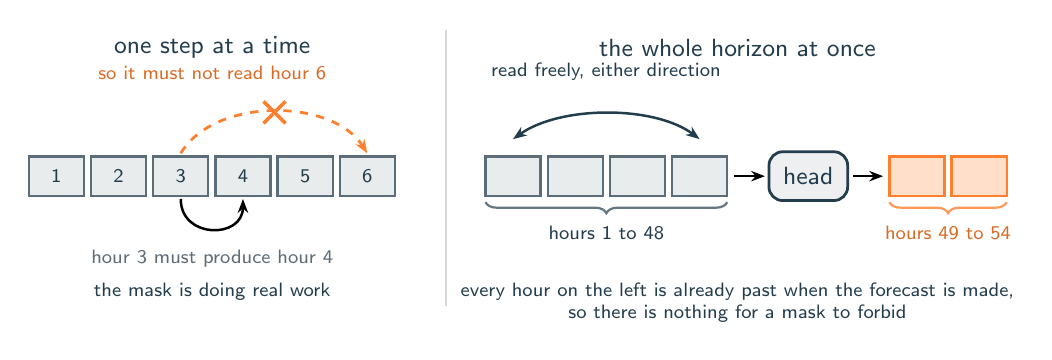
\begin{tikzpicture}[
    every node/.style={font=\sffamily},
    arr/.style={-{Stealth[length=5pt]}, line width=0.9pt, color=c1},
    dbl/.style={{Stealth[length=5pt]}-{Stealth[length=5pt]}, line width=0.9pt, color=c2},
    lab/.style={font=\sffamily\scriptsize, text=labelcolor},
    tag/.style={font=\sffamily\scriptsize, text=c2},
    hot/.style={font=\sffamily\scriptsize, text=c3!85!black},
    tok/.style={rectangle, draw=c2!75, fill=c2!10, line width=0.8pt,
                minimum width=0.70cm, minimum height=0.50cm,
                font=\sffamily\scriptsize, text=c2, inner sep=0pt},
    fut/.style={rectangle, draw=c3, fill=c3!25, line width=0.9pt,
                minimum width=0.70cm, minimum height=0.50cm,
                font=\sffamily\scriptsize, text=c2, inner sep=0pt},
    proc/.style={rectangle, rounded corners=5pt, draw=c2, fill=c2!8, text=c2,
                 line width=1.0pt, font=\sffamily\small},
]

\draw[c2!20, line width=0.8pt] (5.85, 2.30) -- (5.85, 5.80);

% ================================================================ left: one step at a time
\node[tag, font=\sffamily\small] at (2.88, 5.58) {one step at a time};

\foreach \i/\x in {1/0.90, 2/1.69, 3/2.48, 4/3.27, 5/4.06, 6/4.85}{
    \node[tok] at (\x, 3.95) {\i};
}

% what hour 3 is asked to produce
\draw[arr] (2.48, 3.66) .. controls (2.48, 3.15) and (3.27, 3.15) .. (3.27, 3.66);
\node[lab, anchor=north] at (2.88, 3.14) {hour 3 must produce hour 4};

% what it must therefore not read
\draw[c3, line width=1.0pt, dashed, -{Stealth[length=5pt]}]
    (2.48, 4.24) .. controls (2.90, 4.95) and (4.40, 4.95) .. (4.85, 4.24);
\draw[c3, line width=1.3pt] (3.53, 4.62) -- (3.81, 4.90);
\draw[c3, line width=1.3pt] (3.53, 4.90) -- (3.81, 4.62);
\node[hot, anchor=south] at (2.88, 5.05) {so it must not read hour 6};

\node[tag, anchor=north, align=center] at (2.88, 2.72) {the mask is doing real work};

% ================================================================ right: the whole horizon
\node[tag, font=\sffamily\small] at (9.55, 5.58) {the whole horizon at once};

\foreach \x in {6.70, 7.49, 8.28, 9.07}{
    \node[tok] at (\x, 3.95) {};
}
\draw[dbl] (6.70, 4.42) .. controls (7.30, 4.85) and (8.50, 4.85) .. (9.07, 4.42);
\node[tag, anchor=south] at (7.88, 5.05) {read freely, either direction};

\draw[decorate, decoration={brace, amplitude=4pt, mirror}, c2!70, line width=0.8pt]
    (6.35, 3.62) -- (9.42, 3.62)
    node[midway, below=5pt, font=\sffamily\scriptsize, text=c2] {hours 1 to 48};

\draw[arr] (9.50, 3.95) -- (9.90, 3.95);
\node[proc, minimum width=1.0cm, minimum height=0.62cm] at (10.45, 3.95) {head};
\draw[arr] (11.02, 3.95) -- (11.40, 3.95);

\node[fut] at (11.83, 3.95) {};
\node[fut] at (12.62, 3.95) {};
\draw[decorate, decoration={brace, amplitude=4pt, mirror}, c3!80, line width=0.8pt]
    (11.48, 3.62) -- (12.97, 3.62)
    node[midway, below=5pt, font=\sffamily\scriptsize, text=c3!85!black]
    {hours 49 to 54};

\node[tag, anchor=north, align=center] at (9.55, 2.72)
    {every hour on the left is already past when the forecast is made,\\
     so there is nothing for a mask to forbid};

\end{tikzpicture}
\end{document}
